%%%%%%%%%%%%%%%%%%%%%%%%%%%%%%%%%%%%%%%%%%%%%%%%%%%%%%%%%%%%%%%%%%%%%%%%%%%%%%%%
% Appendix-B.tex: Particle tracking
%%%%%%%%%%%%%%%%%%%%%%%%%%%%%%%%%%%%%%%%%%%%%%%%%%%%%%%%%%%%%%%%%%%%%%%%%%%%%%%%
% Outline:
% - Cross-correlation tracking method
% - Fourier transform based orientation analysis
%%%%%%%%%%%%%%%%%%%%%%%%%%%%%%%%%%%%%%%%%%%%%%%%%%%%%%%%%%%%%%%%%%%%%%%%%%%%%%%%
\chapter{Image Analysis Code}

\section{Code Vectorization}
\subsection{Vectorized Code for Spatial Correlation Function}
\label{sec:A-vectorization}
\begin{minted}[frame=lines,framesep=2mm,baselinestretch=1.1,linenos,]{python}
def corrS(X, Y, U, V):
    row, col = X.shape
    vsqrt = (U ** 2 + V ** 2) ** 0.5
    U = U - U.mean()
    V = V - V.mean()
    Ax = U / vsqrt
    Ay = V / vsqrt
    CA = np.ones(X.shape)
    CV = np.ones(X.shape)
    for xin in range(0, col):
        for yin in range(0, row):
            if xin != 0 or yin != 0:
                CA[yin, xin] = (Ax[0:row-yin, 0:col-xin] *
                                Ax[yin:row, xin:col] +
                                Ay[0:row-yin, 0:col-xin] *
                                Ay[yin:row, xin:col]).mean()
                CV[yin, xin] = (U[0:row-yin, 0:col-xin] *
                                U[yin:row, xin:col] +
                                V[0:row-yin, 0:col-xin] *
                                V[yin:row, xin:col]).mean() /
                                (U.std()**2+V.std()**2)
    return CA, CV
\end{minted}

\subsection{Non-vectorized Code for Spatial Correlation Function}
\begin{minted}[frame=lines,framesep=2mm,baselinestretch=1.1,linenos]{python}
def corrS(X, Y, U, V):
    row, col = X.shape
    vsq = 0
    CA = np.zeros((row, col))
    CV = np.zeros((row, col))
    for i in range(0, row):
        for j in  range(0, col):
            vsq += U[i, j]**2 + V[i, j]**2
    for xin in range(0, col):
        for yin in range(0, row):
            count = 0
            CAt = 0
            CVt = 0
            for i in range(0, col-xin):
                for j in range(0, row-yin):
                    ua = U[j, i]
                    va = V[j, i]
                    ub = U[j+yin, i+xin]
                    vb = V[j+yin, i+xin]
                    CAt += (ua*ub+va*vb) / ((ua**2+va**2) *
                            (ub**2+vb**2))**.5
                    CVt += ua*ub + va*vb
                    count += 1
            CA[yin, xin] = CAt / count
            CV[yin, xin] = CVt / vsq
    return CA, CV
\end{minted}


\begin{figure}[!ht]
	\begin{center}
	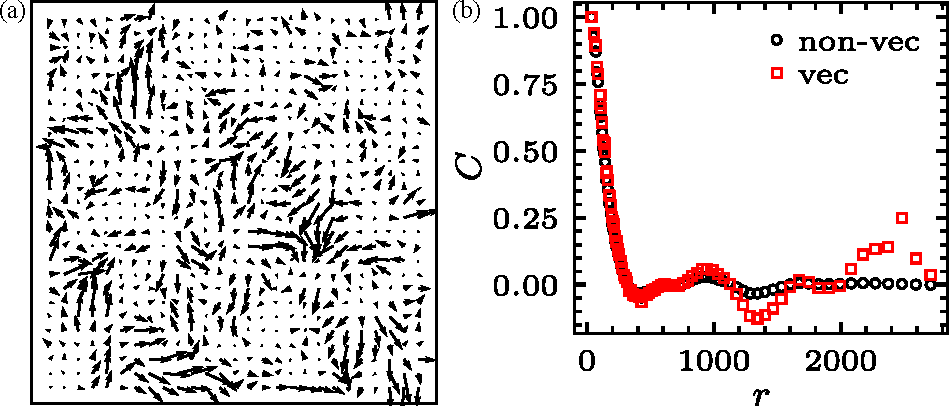
\includegraphics[width=5.5in]{Figs/A-2/vectorization.pdf}
	%select pdftexify command to run jpg or pdf files
	\end{center}
	\caption[The performance of vectorized and non-vectorized code]
	{
	\textbf{The performance of vectorized and non-vectorized code.}
  (a) Sample velocity field.
  (b) Velocity correlation functions obtained from the vectorized and non-vectorized code.
	}
	\label{fig:vectorization-performance}
\end{figure}


\subsection{Performance Comparison}
We notice that the vectorized code has two less nested \texttt{for} loops compared to the non-vectorized code. As a result, the vectorized one runs much faster for the same task. To quantify this performance difference, we perform the spatial correlation function calculation using both code on the same velocity field, shown in Fig.~\ref{fig:vectorization-performance}a. The times taken for the two functions are:
\begin{itemize}
  \item \texttt{Vectorized code: 0.84 s}
  \item \texttt{Non-vectorized code: 52.06 s}
\end{itemize}
The result is shown in Fig.~\ref{fig:vectorization-performance}b. Although in the large $r$ regime, two methods show descrepancies, in the meaningful small $r$ regime, two methods give exactly the same results.


\section{Energy Spectrum Calculation}
\label{sec:A-energy-spectra}
The following code is used for calculating the energy spectra in Chap.~\ref{giant-number-fluctuations-in-3-dimensional-space}.

\begin{minted}[frame=lines,framesep=2mm,baselinestretch=1.1,linenos]{python}
def compute_energy_density(pivData, d=25*0.33, MPP=0.33):
    """
    Compute kinetic energy density in k space from piv data.

    Args:
    pivData -- piv data
    d -- sample spacing
    MPP -- microns per pixel

    Returns:
    E -- kinetic energy field in k space
    """

    row = len(pivData.y.drop_duplicates())
    col = len(pivData.x.drop_duplicates())
    U = np.array(pivData.u).reshape((row, col)) * MPP
    V = np.array(pivData.v).reshape((row, col)) * MPP

    u_fft = np.fft.fft2(U) * d * d
    v_fft = np.fft.fft2(V) * d * d

    E = (u_fft * u_fft.conjugate() + v_fft * v_fft.conjugate()) / 2

    return E

def compute_wavenumber_field(shape, d):
    """
    Compute the wave number field Kx and Ky, and magnitude field k.

    Args:
    shape -- shape of the velocity field and velocity fft field, tuple
    d -- sample spacing.

    Returns:
    k -- wavenumber magnitude field
    K -- wavenumber fields in given dimensions
    """

    for num, length in enumerate(shape):
        kx = np.fft.fftfreq(length, d=d)
        if num == 0:
            k = (kx,)
        else:
            k += (kx,)

    K = np.meshgrid(*k, indexing='ij')

    for num, k1 in enumerate(K):
        if num == 0:
            ksq = k1 ** 2
        else:
            ksq += k1 ** 2

    k_mag = ksq ** 0.5 * 2 * np.pi

    return k_mag, K

def energy_spectrum(pivData, d=25*0.33):
    """
    Compute energy spectrum (E vs k) from pivData.

    Args:
    pivData -- piv data
    d -- sample spacing.

    Returns:
    es -- energy spectrum, DataFrame (k, E)
    """

    row = len(pivData.y.drop_duplicates())
    col = len(pivData.x.drop_duplicates())

    E = compute_energy_density(pivData, d) / (row * d * col * d)
    k, K = compute_wavenumber_field(E.shape, d)

    ind = np.argsort(k.flatten())
    k_plot = k.flatten()[ind]
    E_plot = E.real.flatten()[ind]

    es = pd.DataFrame(data={'k': k_plot, 'E': E_plot})

    return es
\end{minted}

\section{Cross-Correlation Based Particle Detecting Method}
\label{sec:A-cross-correlation-tracking-method}
This is designed for tracking colloidal chains. We show here the basic working principle and the code here. The advantage of this method is that it does not require the feature to be very bright or dark, like traditional particle detecting methods. As long as the features share similar characteristics, i.e. spatial patterns, this method can work well.

\begin{figure}[h]
	\begin{center}
	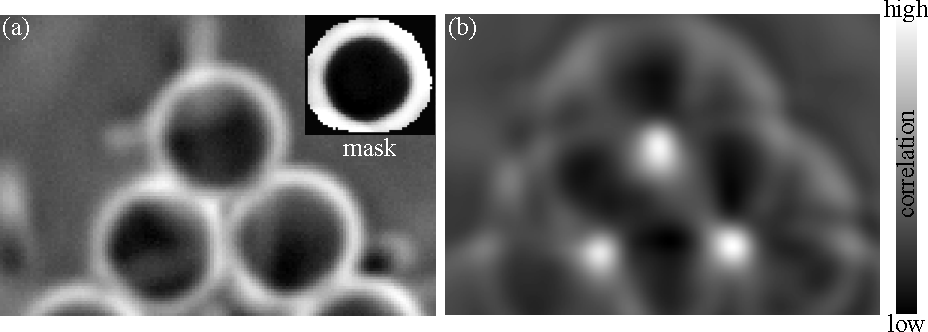
\includegraphics[width=5.5in]{Figs/A-2/corrTrack.pdf}
	%select pdftexify command to run jpg or pdf files
	\end{center}
	\caption[Cross-correlation based particle detecting method]
	{
	\textbf{Cross-correlation based particle detecting method.}
  (a) A sample image of colloidal particles. Inset: a mask produced by cropping the raw image and binarize.
  (b) The cross-correlation map.
	}
	\label{fig:corr-track}
\end{figure}

\subsection{Working Principle}
From raw images, we crop out a single feature which we are looking for as a target mask, as shown in Fig.~\ref{fig:corr-track}a inset. Then, we do a 2D correlation between the target mask and an image (Fig.~\ref{fig:corr-track}a). The resulting correlation map is shown in Fig.~\ref{fig:corr-track}b, where bright pixels stand for high correlation and dark pixels stand for low correlation. The last step is to look for the pixel intensity peaks in the correlation map, as in traditional particle detecting methods.



\subsection{Code}
\begin{minted}[frame=lines,framesep=2mm,baselinestretch=1.1,linenos]{python}
import numpy as np
from scipy.signal import medfilt2d, convolve2d, fftconvolve
from math import exp

def normxcorr2(template, image, mode="full"):
    if np.ndim(template) > np.ndim(image) or \
            len([i for i in range(np.ndim(template)) \
             if template.shape[i] > image.shape[i]]) > 0:
    template = template - np.mean(template)
    image = image - np.mean(image)
    a1 = np.ones(template.shape)
    ar = np.flipud(np.fliplr(template))
    out = fftconvolve(image, ar.conj(), mode=mode)
    image = fftconvolve(np.square(image), a1, mode=mode) - \
            np.square(fftconvolve(image, a1, mode=mode)) \
            / (np.prod(template.shape))
    image[np.where(image < 0)] = 0
    template = np.sum(np.square(template))
    out = out / np.sqrt(image * template)
    out[np.where(np.logical_not(np.isfinite(out)))] = 0
    return -out

def matlab_style_gauss2D(shape=(3,3),sigma=0.5):
    m,n = [(ss-1.)/2. for ss in shape]
    y,x = np.ogrid[-m:m+1,-n:n+1]
    h = np.exp( -(x*x + y*y) / (2.*sigma*sigma) )
    h[ h < np.finfo(h.dtype).eps*h.max() ] = 0
    sumh = h.sum()
    if sumh != 0:
        h /= sumh
    return h

def FastPeakFind(data):
    if str(data.dtype) != 'float32':
        data = data.astype('float32')
    mf = medfilt2d(data, kernel_size=3)
    mf = mf.astype('float32')
    thres = max(min(np.amax(mf,axis=0)), min(np.amax(mf,axis=1)))
    filt = matlab_style_gauss2D()
    conv = convolve2d(mf, filt, mode='same')
    w_idx = conv > thres
    bw = conv.copy()
    bw[w_idx] = 1
    bw[~w_idx] = 0
    thresholded = np.multiply(bw, conv)
    edg = 3
    shape = data.shape
    idx = np.nonzero(thresholded[edg-1: shape[0]-edg-1, \
                    edg-1: shape[1]-edg-1])
    idx = np.transpose(idx)
    cent = []
    for xy in idx:
        x = xy[0]
        y = xy[1]
        if thresholded[x, y] >= thresholded[x-1, y-1] and \
            thresholded[x, y] > thresholded[x-1, y] and \
            thresholded[x, y] >= thresholded[x-1, y+1] and \
            thresholded[x, y] > thresholded[x, y-1] and \
            thresholded[x, y] > thresholded[x, y+1] and \
            thresholded[x, y] >= thresholded[x+1, y-1] and \
            thresholded[x, y] > thresholded[x+1, y] and \
            thresholded[x, y] >= thresholded[x+1, y+1]:
            cent.append(xy)
    cent = np.asarray(cent).transpose()
    return cent

def maxk(array, num_max):
    array = np.asarray(array)
    length = array.size
    array = array.reshape((1, length))
    idx = np.argsort(array)
    idx2 = np.flip(idx)
    return idx2[0, 0:num_max]

def gauss1(x,a,x0,sigma):
    return a*exp(-(x-x0)**2/(2*sigma**2))

def track_spheres(img, mask, num_particles):
    def gauss1(x,a,x0,sigma):
        return a*exp(-(x-x0)**2/(2*sigma**2))
    corr = normxcorr2(mask, img, mode='same')
    cent = FastPeakFind(corr)
    peaks = corr[cent[0], cent[1]]
    ind = maxk(peaks, num_particles)
    max_coor_tmp = cent[:, ind]
    max_coor = max_coor_tmp.astype('float32')
    pk_value = peaks[ind]
    for num in range(0, num_particles):
        x = max_coor_tmp[0, num]
        y = max_coor_tmp[1, num]
        fitx1 = np.asarray(range(x-7, x+8))
        fity1 = np.asarray(corr[range(x-7, x+8), y])
        popt, pcov = curve_fit(gauss1, fitx1, fity1, p0=[1, x, 3])
        max_coor[0, num] = popt[1]
        fitx2 = np.asarray(range(y-7, y+8))
        fity2 = np.asarray(corr[x, range(y-7, y+8)])
        popt,pcov = curve_fit(gauss1, fitx2, fity2, p0=[1, y, 3])
        max_coor[1, num] = popt[1]
    return max_coor, pk_value
\end{minted}


\section{Fourier Transform Based Orientation Analysis}
\label{sec:A-fourier-transform-based-orientation-analysis}
\subsection{Working Principle}
The orientation of patterns in an image can be found by calculating the Fourier transform of the image. The idea is that in the direction of predominant pattern orientation (Fig.~\ref{fig:oft-illustration}a, the vertical direction), the signal frequency is smaller compared to the perpendicular direction. Such feature manifests in the frequency domain as anisotropic patterns (Fig.~\ref{fig:oft-illustration}b, horizontal orientation). This method is used in the study of the emergence of active turbulence in Chap.~\ref{the-emergence-of-active-turbulence}.

\begin{figure}[h]
	\begin{center}
	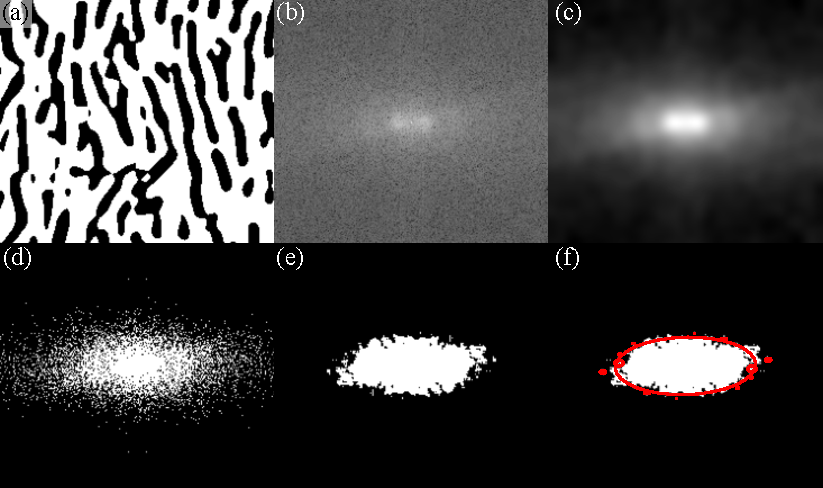
\includegraphics[width=5.5in]{Figs/A-2/orientationFT.pdf}
	%select pdftexify command to run jpg or pdf files
	\end{center}
	\caption[Fourier transform based orientation analysis illustration]
	{
	\textbf{Fourier transform based orientation analysis illustration.}
  (a) Raw image.
  (b) Fourier transformed image.
  (c) Smoothing.
  (d) Binarization.
  (e) Despeckling.
  (f) Pattern detection.
	}
	\label{fig:oft-illustration}
\end{figure}

The procedures are illustrated in Fig.~\ref{fig:oft-illustration}. We first perform Fourier transform on the raw image (Fig.~\ref{fig:oft-illustration}a), then smooth this transformed image (Fig.~\ref{fig:oft-illustration}b) using a Gaussian filter to get Fig.~\ref{fig:oft-illustration}c, which is then binarized using a ``isodata'' threshold, yielding Fig.~\ref{fig:oft-illustration}d. A median filter is applied on the binarized image to remove small noise, known as despeckling, to obtain Fig.~\ref{fig:oft-illustration}e. Finally, we detect the anisotropic pattern in Fig.~\ref{fig:oft-illustration}e using a Python function \texttt{skimage.measure.regionprops}. Red circles in Fig.~\ref{fig:oft-illustration}f indicate all the patterns detected in the image, and we take the biggest one to examine the orientation. The Python implementation of these procedures is shown in Sec.~\ref{sec:oft-code}. Some example results are shown in Sec.~\ref{sec:oft-gallery}.

\subsection{Code}
\label{sec:oft-code}

\begin{minted}[frame=lines,framesep=2mm,baselinestretch=1.1,linenos]{python}
from skimage import measure, filters
import pandas as pd
from scipy.ndimage import gaussian_filter, median_filter

def sectionWindow(imgShape, windowShape):
    Xnum = math.floor(imgShape[0]/windowShape[0])
    Ynum = math.floor(imgShape[1]/windowShape[1])
    Xrem = imgShape[0]%windowShape[0]
    Yrem = imgShape[1]%windowShape[1]
    Xstart = math.floor(Xrem/2)
    Ystart = math.floor(Yrem/2)
    Xend = imgShape[0] - Xstart + 1
    Yend = imgShape[1] - Ystart + 1
    X = np.asarray(range(Xstart, Xend, windowShape[0]))
    Y = np.asarray(range(Ystart, Yend, windowShape[1]))
    return X, Y

def getOrientation(bw_img):
    label_img = measure.label(thres)
    prop = measure.regionprops_table(label_img,
                    properties=['area', 'major_axis_length',
                    'minor_axis_length', 'orientation'])
    prop_df = pd.DataFrame(prop)
    if len(prop_df) == 0:
        return 0, 0
    else:
        main_feature = prop_df.sort_values(by='area', \
                                ascending=False).iloc[0]
        return main_feature.orientation,
              main_feature.major_axis_length / \
              main_feature.minor_axis_length

# test code
windowShape = (50, 50)
img = io.imread(r'..\img\testFT_4.jpg', as_gray=True)
X, Y = sectionWindow(img.shape, windowShape)
y = X[0:X.size-1] + windowShape[0]/2
x = Y[0:Y.size-1] + windowShape[1]/2
x, y = np.meshgrid(x, y)
u_ori = x.copy()
v_ori = y.copy()
for i in range(0, x.shape[0]):
    for j in range(0, y.shape[1]):
        window = img[X[i]:X[i+1], Y[j]:Y[j+1]]
        fft = np.log(abs(np.fft.fft2(window)))
        fft = np.fft.fftshift(fft) ## 1
        smooth = gaussian_filter(fft, 5) ## 2
        thres = smooth > filters.threshold_isodata(smooth) ## 3
        despeck = median_filter(thres, size=5) ## 4
        ori, orim = getOrientation(despeck) ## 5
        u_ori[i, j] = orim*math.cos(ori)
        v_ori[i, j] = orim*math.sin(ori)

plt.figure(dpi=300)
plt.imshow(img, cmap='gray')
plt.quiver(x, y, u_ori, v_ori, color='red')
plt.axis('off')
\end{minted}

\subsection{Some Examples}
\label{sec:oft-gallery}
Some example applications of this method is shown in Fig.~\ref{fig:oft-gallery}

\begin{figure}[h]
	\begin{center}
	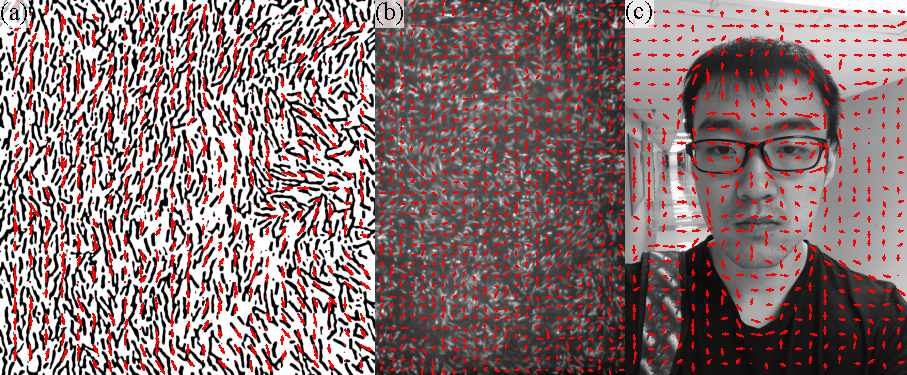
\includegraphics[width=5.5in]{Figs/A-2/oft-gallery.pdf}
	%select pdftexify command to run jpg or pdf files
	\end{center}
	\caption[Fourier transform based orientation analysis examples]
	{
	\textbf{Fourier transform based orientation analysis examples.}
  Orientations of
  (a) a synthesized pattern,
  (b) an image of bacterial suspensions and
  (c) a photo of me.
	}
	\label{fig:oft-gallery}
\end{figure}

\section{Density Fluctuation Calculations}
\label{sec:A-df-calculation}
The principles of density fluctuation calculation has already been described in Chap.~\ref{giant-number-fluctuations-in-3-dimensional-space}. Here, I show the Python implementation of the calculation.

\begin{minted}[frame=lines,framesep=2mm,baselinestretch=1.1,linenos]{python}
def df2(img_stack, boxsize=None, size_min=5, step=250):
    """
    Compute number fluctuations of an image stack.

    Args:
    img_stack -- a stack of image, a 3D array
    boxsize -- the subsystem size to look at.
    size_min -- the smallest box size
    step -- step used when dividing image into windows

    Returns:
    df -- DataFrame of n and d,
          where n is box area (px^2) and
          d is total number fluctuations (box_area*dI)
    """
    L = min(img_stack.shape[1:3])
    if boxsize == None:
        boxsize = np.unique(np.floor(
                np.logspace(np.log10(size_min), np.log10(L/2), 100)))

    dI_list = []
    for bs in boxsize:
        I = divide_stack(img_stack, winsize=[bs, bs], step=step)
        dI = I.std(axis=0).mean() * bs ** 2
        dI_list.append(dI)

    return pd.DataFrame({'n': np.array(boxsize)**2, 'd': dI_list})
\end{minted}
